\section{MPI One-Sided Communication}
\subsection{Required submission files}
\begin{enumerate}
  \item \hl{The updated \emph{gauss.c} file.}

  \item \hl{The new performance plots and description in the report.}

\end{enumerate}

\subsection{Questions}
\begin{enumerate}
  \item \hl{Which MPI-IO operations were applied to transform the code? Explain your choices.}
  
  \item \hl{What is "Data Sieving" and "2-Phase IO"? How do they help improve IO
performance?}

  \item \hl{Was the original implementation scalable in terms of IO performance?}
  
  \item \hl{Was the original implementation scalable in terms of RAM storage?}
  
  \item \hl{How much of the communication in the application was replaced or eliminated with MPI-IO? (Use
Vampir)}

  \item \hl{Were there any performance improvements due to the change to MPI-IO?}

\end{enumerate}
% % Figure example
% \begin{figure}[p] % h=here, t=top, b=bottom, p=(extra)page, !=force
%    \begin{center}
%      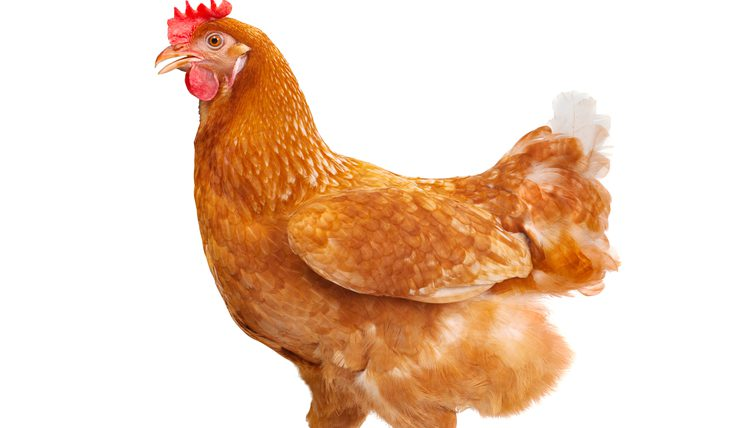
\includegraphics[width=.9\linewidth]{figure.png} % It searches in the Figures/ folder!
%      \caption{Caption text}
%      \label{fig:figureLabelName}
%    \end{center}
% \end{figure}
